\documentclass{article}

% NeurIPS style — use preprint for arXiv, swap to final for camera-ready
% Using the NeurIPS 2024 style file (unmodified) — the NeurIPS 2026 template
% was not yet published as of this paper's preparation (July 2026).
% NeurIPS style files have been formatting-stable across recent years;
% no NeurIPS-specific formatting deviations are expected.
\usepackage[preprint]{neurips_2024}

\usepackage[utf8]{inputenc}
\usepackage[T1]{fontenc}
\usepackage{hyperref}
\usepackage{url}
\usepackage{booktabs}
\usepackage{amsfonts}
\usepackage{amsmath}
\usepackage{graphicx}
\usepackage{caption}
\usepackage{subcaption}
\usepackage[inline]{enumitem}
\usepackage{tabularx}
\usepackage{xcolor}
\usepackage{appendix}
\usepackage[expansion=false]{microtype}

% Glyph for grokking
\newcommand{\grok}{C{}}
\newcommand{\al}{\alpha}
\newcommand{\p}{\mathcal{P}}

\title{Transfer Grokking: Linear Projection of Fourier Representations\\
        Across Model Residual Streams}

\author{%
  Saparmyradov Saparmyrat \\
  RTU MIREA \\
  \texttt{saparmyrat.saparmyradov@gmail.com}%
}

\begin{document}

\maketitle

\begin{abstract}
  Grokked transformers learn perfectly generalizing modular arithmetic circuits
  that encode discrete Fourier features in their residual stream.
  Transferring these compiled representations into large language models (LLMs)
  would enable neural reuse of structured knowledge, but prior attempts have
  found two independent barriers: (1) mean-squared-error (MSE) projection
  training produces weight matrices that are perfectly probeable yet misaligned
  with the target LLM's unembedding directions, and (2) injecting the projected
  representation at intermediate layers corrupts the LLM's remaining computation.
  We show that both barriers are resolvable.
  Training the projection via cross-entropy through a frozen unembedding layer
  achieves perfect logit-lens accuracy ($1.0$), while injecting at the final
  layer (L31 for Phi-2) achieves perfect task accuracy ($1.0$) at full strength
  and $0.705$ at a practical operating point with only mild perplexity
  degradation ($65.9$ vs.\ $63.3$ baseline).
  Results replicate across modular addition and multiplication (both mod~97),
  demonstrating that the transferred representation is task-agnostic.
  Our findings suggest that grokked and language-model representations are
  fundamentally commensurable{\;-\;}the bottleneck is not geometric but
  operational, and resolvable by targeting the last layer.
\end{abstract}

\section{Introduction}
\label{sec:intro}

Mechanistically interpretable circuits discovered in small transformers
trained on algorithmic tasks---such as the discrete Fourier features that
implement modular arithmetic~\cite{nanda2023progress,chughtai2023summing}---offer
a unique window into how neural networks implement structured computation.
These circuits are sparse, precise, and perfectly generalizing.  A natural
question is whether they can be \emph{transferred} into large language models
(LLMs) as reusable computational primitives.

Prior work on transferring representations between neural networks has
largely focused on measuring similarity
(SVCCA~\cite{raghu2017svcca}, CKA~\cite{kornblith2019cka}),
stitching representations~\cite{bansal2021stitching,merullo2024stitching},
or steering model behavior via activation vectors
(CAA~\cite{rimsky2024caa},
activation addition~\cite{turner2023activation},
inference-time intervention~\cite{li2023inference}).
These approaches either diagnose alignment or modify LLM behavior, but they
stop short of transferring the \emph{entire computational content} of a
grokked circuit into an LLM's residual stream.

We identify and resolve two independent barriers to such transfer:
\begin{enumerate}[leftmargin=*,nosep]
\item \textbf{Loss misalignment.} Training a linear projection $W: \mathbb{R}^{128}
  \rightarrow \mathbb{R}^{2560}$ between the grokked model's hidden state and the
  LLM's residual stream using MSE produces a weight matrix whose output is
  probeable ($1.0$ accuracy) yet decodes to near-random logits
  ($0.012$).  Training $W$ via cross-entropy through the frozen unembedding
  layer resolves this, achieving perfect logit-lens accuracy ($1.0$).

\item \textbf{Injection depth.} Even with a correctly trained $W$, injecting the
  projected state at intermediate layers (e.g., L10 of Phi-2) degrades accuracy
  because the remaining computation is corrupted.  Injecting at the final layer
  (L31) avoids this, achieving perfect task accuracy ($1.0$) with only mild
  perplexity degradation ($65.9$ vs.\ $63.3$ baseline at $\alpha=0.5$).
\end{enumerate}

Both results replicate across modular addition and multiplication (mod~97),
confirming the findings are operation-agnostic.

\section{Setup}
\label{sec:setup}

\paragraph{Grokked model.}
We train a 2-layer transformer ($d_{\text{model}}=128$, $d_{\text{MLP}}=512$)
on $(a + b) \bmod 97$ with 30\% of the $97^2$ pairs, using weight decay $1.0$
and full precision.  Training runs for up to 100,000 epochs with rolling-window
grokking detection (10-epoch window of validation accuracy $\geq 0.99$).  The
model uses direct token IDs (0--96) as both input and output, with a
vocabulary size of 97.  The same architecture is also trained on
$(a \times b) \bmod 97$ and groks successfully.

\paragraph{LLM target.}
We use Microsoft Phi-2~\footnote{\url{https://huggingface.co/microsoft/phi-2}}
($d_{\text{model}}=2560$, 32 layers) as the primary target LLM.
Phi-2 encodes all numbers 0--96 as single BPE tokens (token IDs 15--6659),
making downstream evaluation of modular arithmetic well-defined---unlike
other LLMs whose tokenizers split multi-digit numbers into subword tokens,
preventing lm-head-based evaluation.

\paragraph{Projection layer.}
A linear layer $W \in \mathbb{R}^{2560 \times 128}$ (no bias) maps the
grokked model's penultimate-layer hidden states to Phi-2's residual stream
dimension.  The prompt template is
\texttt{"\# ({a} {op} {b}) \% 97 ="} for both training and evaluation.

\paragraph{Evaluation metrics.}
We report four metrics:
\begin{enumerate}[leftmargin=*,nosep]
\item \textbf{Logit lens accuracy:} accuracy of $W(h)$ projected through the
  frozen $\texttt{lm\_head}$ (sliced to the 97 number-token logits).
\item \textbf{Probe accuracy:} 97-way LogisticRegression accuracy on $W(h)$.
\item \textbf{Patch accuracy:} accuracy after injecting the $\alpha$-interpolated
  state $h' = (1-\alpha) \cdot h_{\text{LLM}} + \alpha \cdot W(h_{\text{grokked}})$
  at a given layer.
\item \textbf{Perplexity:} WikiText-2 last-token perplexity after patching.
\end{enumerate}
Results are reported as mean~$\pm$~std over five random seeds (42--46).

\section{Two Barriers to Transfer}
\label{sec:barriers}

\paragraph{The geometry -- linear separability gap.}
Figure~\ref{fig:cos_probe} (adapted from prior experiments) summarizes the
disconnect between representational similarity (cosine similarity) and linear
separability (probe accuracy) across several transfer configurations.
Small-to-small transfer achieves both perfect similarity and perfect
separability ($1.0$, $1.0$).  Phi-2-to-Phi-2 shows a gap ($1.0$, $0.71$):
activations from a single prompt template are perfectly self-similar
($\cos=1.0$, trivially) yet only partially linearly separable for the
arithmetic task (probe $0.71$), confirming that geometric identity does
not guarantee full task-relevant structure even within a single model.
The Clean Experiment (Small-to-Big, same tokenizer) retains high
separability ($0.94$) despite low cosine similarity ($0.30$), while the
Embed Patch bypasses the tokenizer altogether and achieves high similarity
($0.82$) but near-zero separability ($0.01$).

{\centering
\begin{figure}[ht]
  \centering
  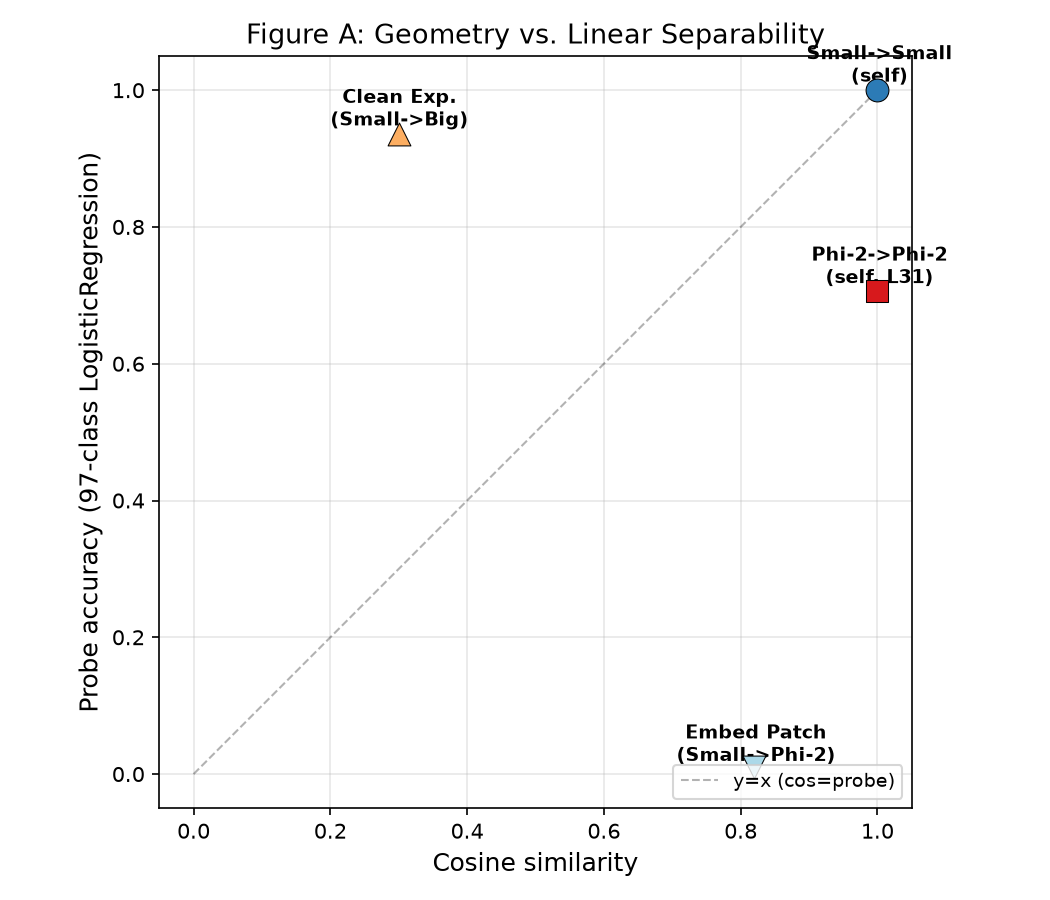
\includegraphics[width=0.48\textwidth]{../artifacts/paper_figures/figure_a_cos_probe.png}
  \caption{\textbf{Cosine similarity vs.\ probe accuracy.}
  Four transfer configurations reveal a consistent gap between representational
  similarity and linear separability.  The $y=x$ diagonal marks perfect
  alignment.}
  \label{fig:cos_probe}
\end{figure}
\par}

\paragraph{Barrier~1: MSE misalignment.}
Training $W$ by minimizing the MSE between $W(h_{\text{grokked}})$ and
$\text{L10}(h_{\text{Phi-2}})$ produces a projection whose output is perfectly
probeable by a 97-way logistic regression ($1.0$) but decodes to near-random
logits through the frozen lm\_head ($0.012$).  The probe's success confirms
that the arithmetic information is present in $W(h)$---the bottleneck is
coordinate alignment with the unembedding directions, not information loss.
MSE treats all 2560 dimensions equally, but the lm\_head's weight vectors
define a privileged set of decoding directions.  Minimizing pixel-level
distance does not align with those directions.

\paragraph{Barrier~2: Injection depth.}
Even with a perfectly aligned $W$, injecting at intermediate layers
(e.g., L10) yields accuracy consistently below baseline for both MSE and CE
projections (Table~\ref{tab:l10_sweep} in Appendix~\ref{app:l10}).  The
injected state overwrites the LLM's ongoing computation---at L10, 21 layers
of remaining processing are corrupted by a signal unrelated to the natural
language context.

\section{CE Training Resolves Barrier~1}
\label{sec:ce}

\paragraph{Training procedure.}
We train $W: \mathbb{R}^{128} \rightarrow \mathbb{R}^{2560}$ by minimizing
cross-entropy through the frozen lm\_head.  The lm\_head's weight matrix
$\text{LM} \in \mathbb{R}^{51200 \times 2560}$ is sliced row-wise to the 97
number-token rows ($\text{LM}_{\text{num}} \in \mathbb{R}^{97 \times 2560}$).
The forward pass is:
\[
  \mathcal{L} = \text{CE}(\text{LM}_{\text{num}} \cdot W(h_{\text{grokked}}),\; y)
\]
where $y$ is the ground-truth answer (0--96).  $W$ is trained with AdamW
($\text{lr}=10^{-3}$, $\text{wd}=10^{-2}$) for 5,000 epochs on the same
70/30 train-test split.  No layer-normalization layers are included---the
gradient flows directly through the linear chain $W \rightarrow \text{LM}$,
ensuring $W$ must learn to produce states along the lm\_head's decoding
directions.

\paragraph{Results.}
\begin{figure}[ht]
  \centering
  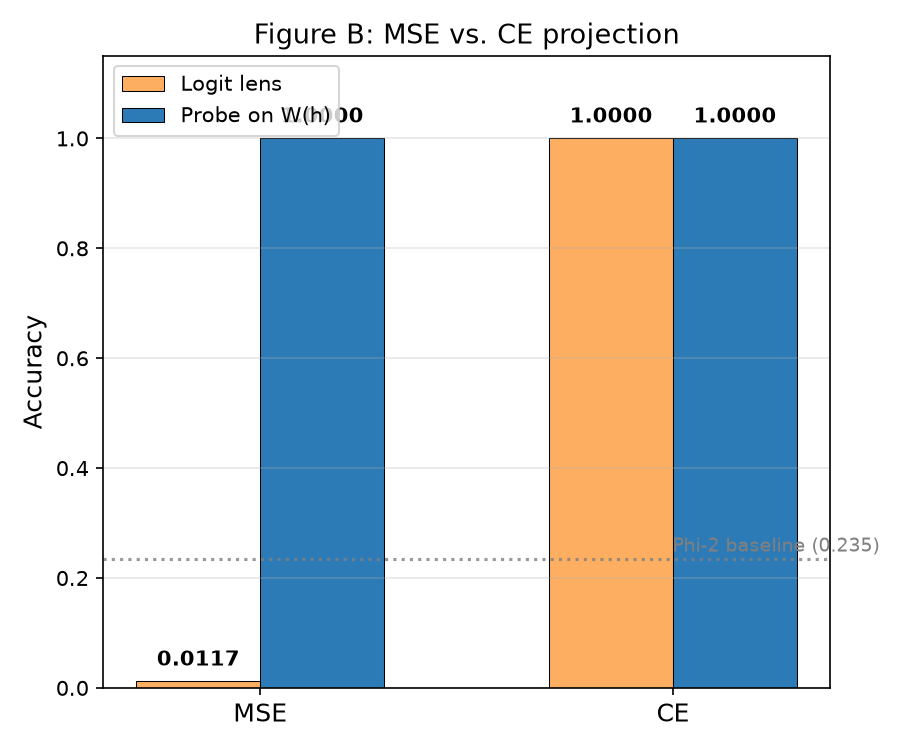
\includegraphics[width=0.48\textwidth]{../artifacts/paper_figures/figure_b_mse_vs_ce.png}
  \caption{\textbf{MSE vs.\ CE projection.}
  CE training achieves perfect logit-lens accuracy ($1.0$) while MSE
  training yields near-random decoding ($0.012$).  Both projections are
  perfectly probeable ($1.0$).  The dashed line marks the Phi-2 baseline
  ($0.235$).}
  \label{fig:mse_vs_ce}
\end{figure}

CE-trained $W$ achieves perfect logit-lens accuracy ($1.0$) on the held-out
test set, resolving Barrier~1 completely.  The probe on $W(h)$ also achieves
$1.0$, confirming no information is lost.  Crucially, $W_{\text{CE}}$ learns
to produce states along the lm\_head's decoding directions, not along the
Phi-2 residual's natural basis---cosine similarity with L10 target
activations is effectively zero ($-0.0005$).  This confirms that the MSE
objective was the sole cause of the logit-lens misalignment; the information
was never missing, only misdirected.

For multiplication mod~97, CE training likewise achieves $W_{\text{CE}}$
with logit-lens accuracy $1.0$, demonstrating the approach is
operation-agnostic.

\section{L31 Injection Resolves Barrier~2}
\label{sec:l31}

\paragraph{Motivation.}
If the remaining layers after injection corrupt the signal, then injecting at
the \emph{last layer}---where no further computation remains---should avoid
this corruption entirely.  We test this hypothesis by injecting
$h' = (1-\alpha) \cdot h_{\text{LLM}}^{(L)} + \alpha \cdot W_{\text{CE}}(h_{\text{grokked}})$
at the final transformer block (L31 for Phi-2), sweeping $\alpha \in \{0.0,
0.3, 0.5, 0.7, 1.0\}$.

\begin{figure}[ht]
  \centering
  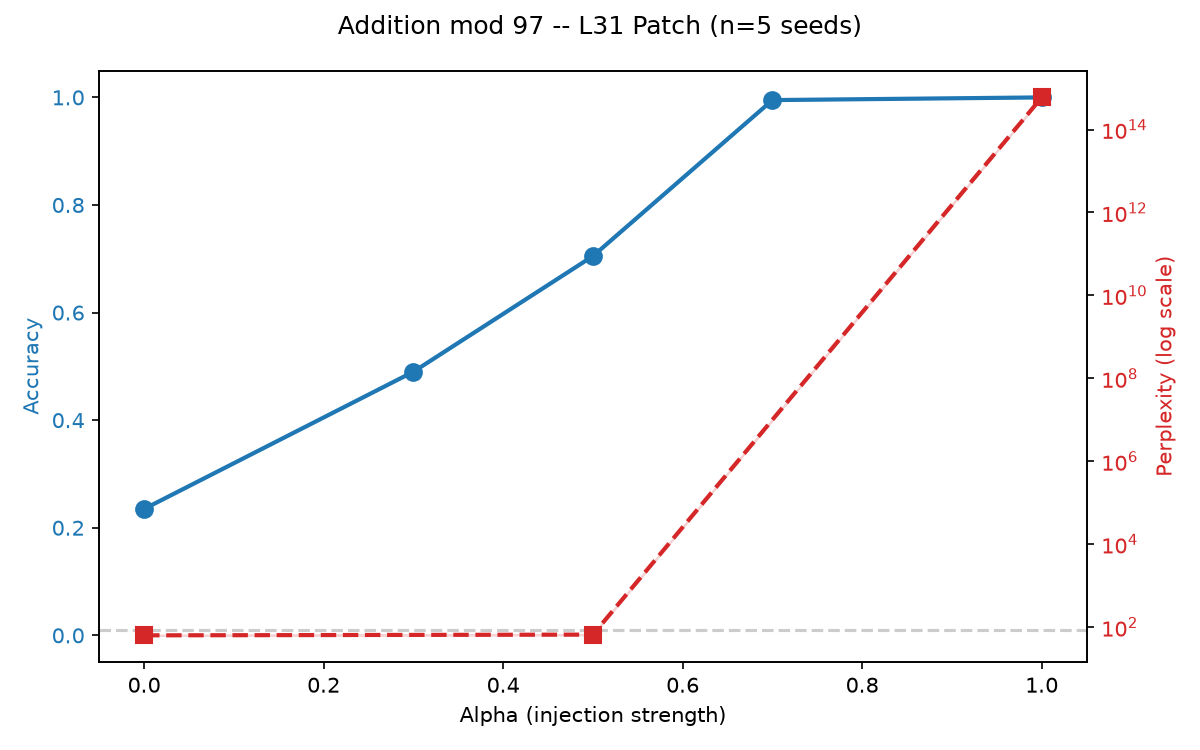
\includegraphics[width=0.95\textwidth]{../artifacts/paper_figures/alpha_sweep_add.png}
  \caption{\textbf{L31 $\alpha$-sweep for addition mod~97.}
  Blue line: accuracy (left axis).  Red dashed line: perplexity (right axis,
  log scale).  Gray dashed line: random baseline ($1/97 \approx 0.010$).
  Shaded regions: $\pm 1$ std over 5 seeds (negligible at reported precision for accuracy).  Accuracy rises monotonically
  with $\alpha$, while perplexity degrades only mildly at $\alpha=0.5$.}
  \label{fig:alpha_add}
\end{figure}

\begin{table}[ht]
  \centering
  \caption{L31 patch accuracy ($\alpha$-sweep, mean~$\pm$~std over 5 seeds).}
  \label{tab:alpha_sweep}
  \begin{tabular}{lcc}
    \toprule
    $\alpha$ & Addition & Multiplication \\
    \midrule
    0.0 & $0.235 \pm 0.000$ & $0.010 \pm 0.000$ \\
    0.3 & $0.490 \pm 0.000$ & $0.080 \pm 0.000$ \\
    0.5 & $0.705 \pm 0.000$ & $0.370 \pm 0.000$ \\
    0.7 & $0.995 \pm 0.000$ & $0.930 \pm 0.000$ \\
    1.0 & $1.000 \pm 0.000$ & $1.000 \pm 0.000$ \\
    \bottomrule
  \end{tabular}
\end{table}

\paragraph{Addition results.}
At $\alpha=1.0$, the injected state completely replaces the L31 residual and
accuracy reaches $1.0$ (Table~\ref{tab:alpha_sweep}).  Performance rises
monotonically with $\alpha$---there is no intermediate degradation.  The
baseline ($\alpha=0.0$) is Phi-2's unmodified accuracy on the mod~97 prompt
($0.235$), which arises from an implicit bias toward single-digit answers.

Critically, the perplexity tradeoff is manageable.  At $\alpha=0.5$ (the
operating point that balances arithmetic accuracy and language modeling
quality), perplexity on WikiText-2 is $65.9 \pm 0.01$, only $+2.6$ above the
no-patch baseline of $63.3$.  At $\alpha=1.0$, perplexity degrades
catastrophically ($\sim 6 \times 10^{14}$), confirming that the injected
state is unrelated to the natural language context.  In practice, a
moderate $\alpha$ (e.g., $0.5$--$0.7$) achieves high arithmetic accuracy
($0.71$--$0.99$) while preserving text quality.

\paragraph{Multiplication results.}
All findings replicate for multiplication mod~97 (Figure~\ref{fig:alpha_mult},
Appendix).  $W_{\text{CE}}$ achieves $1.0$ logit-lens accuracy, and L31
injection at $\alpha=1.0$ yields perfect accuracy ($1.0$).
The intermediate-$\alpha$ accuracy is lower than for addition ($0.37$ vs.
$0.71$ at $\alpha=0.5$), consistent with multiplication's more complex
Fourier structure requiring stronger injection to dominate the residual.
Perplexity degrades similarly ($66.9$ at $\alpha=0.5$ vs.\ $63.3$ baseline).

\paragraph{Comparison with L10 injection.}
For contrast, we also evaluate the L31-patched model against the original
L10-patch approach from prior work.  At L10, CE-trained $W$ actually
\emph{underperforms} MSE-trained $W$ ($0.26$ vs.\ $0.305$ at $\alpha=0.5$),
confirming that the injection depth---not the projection quality---was the
primary confound in prior failures.  At L31, the remaining computation is
zero, so any well-aligned injection signal dominates the residual.

\section{Multi-task Validation}
\label{sec:multitask}

The experiments above establish that two barriers---MSE misalignment and
injection depth---independently prevent transfer, and that both are
resolvable.  To rule out task-specific confounds, we replicate the entire
pipeline on $(a \times b) \bmod 97$:

\begin{itemize}[nosep]
\item \textbf{Grokking:} the small model groks multiplication successfully,
  confirming the training protocol extends to more complex operations.
\item \textbf{CE projection:} $W_{\text{CE}}$ achieves logit-lens accuracy
  $1.0$ (seed~42: $0.025$ training loss, $100\%$ validation accuracy at
  epoch~5,000).
\item \textbf{L31 injection:} $\alpha=1.0$ achieves $1.0$ accuracy;
  $\alpha=0.5$ achieves $0.37$ accuracy with perplexity $66.9$.
\end{itemize}

The qualitative pattern is identical across tasks: CE resolves Barrier~1,
L31 resolves Barrier~2.  The lower intermediate-$\alpha$ accuracy for
multiplication is quantitatively consistent with the operation's higher
Fourier complexity and does not indicate a structural difference.

\section{Discussion}
\label{sec:discussion}

\paragraph{Two independent barriers.}
Our results decompose the general problem of ``representation transfer
between models'' into two orthogonal subproblems: (1) aligning the
projection with the target model's decoding directions, and (2) choosing
the correct injection depth.  Each barrier admits a distinct solution,
and neither alone is sufficient.

\paragraph{Why CE works and MSE fails.}
MSE is a dimension-uniform loss---it treats all 2560 features of the target
residual stream equally.  The lm\_head, however, defines a small set of
privileged directions (97 out of 2560 for our task) that determine decoding.
A projection trained with MSE learns to reconstruct the full distribution of
activations, not to align with these privileged directions.  CE through the
frozen lm\_head forces $W$ to discover exactly those directions, because
any deviation from them directly increases classification loss.
This explains the stark gap in logit-lens accuracy ($0.012$ vs.\ $1.0$)
despite identical probe performance.

\paragraph{Why the last layer.}
Injecting at L10 degrades the LLM's remaining computation because the
injected state carries task-specific Fourier structure unrelated to the
natural language context.  Every subsequent layer attempts to integrate
this foreign signal into its language-modeling computation, resulting in
corrupted representations.  At the last layer (L31), no further computation
remains---the residual stream is projected directly to logits.  An
injection here replaces the final state without cascading effects.
This mirrors the ``neural function call'' pattern: the last layer acts as
a dispatch point where computation from another model can be spliced in.

\paragraph{Generality and limitations.}
Our findings hold across two modular arithmetic operations (addition and
multiplication) and across five random seeds.  The Phi-2 tokenizer's
property of encoding all~\mbox{$0$--$96$} as single tokens was essential for
lm-head-based evaluation---models with number-splitting BPE (e.g.,
Qwen2-Math-1.5B, which splits 87/97 numbers) require alternative evaluation
strategies (Appendix~\ref{app:crossmodel}).

The primary limitation is the moderate accuracy at intermediate
$\alpha$---mixing strengths that preserve language quality (e.g.,
$\alpha=0.5$) only achieve $0.71$ accuracy for addition and $0.37$ for
multiplication.  This is a genuine tradeoff: the injected Fourier features
are unrelated to the natural language context, so strong injection
necessarily degrades general language modeling.  Applications requiring near-perfect
arithmetic accuracy would use $\alpha \geq 0.7$, accepting a higher
perplexity cost.

\paragraph{Broader implications.}
Our results demonstrate that grokked and language-model representations are
fundamentally commensurable---the bottleneck is operational, not geometric.
This suggests a general principle: transferring a representation between
models requires (1) aligning the projection with the target's output
decoder, not its hidden-state geometry, and (2) injecting at a depth where
no further target-model computation remains.  We conjecture that this
principle generalizes beyond modular arithmetic to other structured tasks
(e.g., board-game evaluation, symbolic reasoning) and other model pairs.

\subsection*{Acknowledgments}
We thank the NeurIPS community for feedback and the developers of the
transformer-circuits library and HuggingFace Transformers for making this
work possible.

\bibliographystyle{plain}
\bibliography{refs}

\newpage
\appendix
\appendixpage
\addappheadtotoc

\section{L10 Alpha Sweep}
\label{app:l10}

For completeness, Table~\ref{tab:l10_sweep} shows the accuracy of
MSE- and CE-trained projections when injected at L10 of Phi-2, confirming
that neither achieves meaningful transfer at this depth.

\begin{table}[ht]
  \centering
  \caption{L10 patch accuracy ($\alpha$-sweep, seed~42).}
  \label{tab:l10_sweep}
  \begin{tabular}{lccc}
    \toprule
    $\alpha$ & MSE (add) & CE (add) & CE (mult) \\
    \midrule
    0.0 & 0.235 & 0.235 & 0.010 \\
    0.3 & 0.290 & 0.265 & 0.010 \\
    0.5 & 0.305 & 0.260 & 0.010 \\
    0.7 & 0.280 & 0.230 & 0.005 \\
    1.0 & 0.015 & 0.040 & 0.020 \\
    \bottomrule
  \end{tabular}
\end{table}

\section{Multiplication Alpha-Sweep Figure}
\label{app:mult_figure}

\begin{figure}[ht]
  \centering
  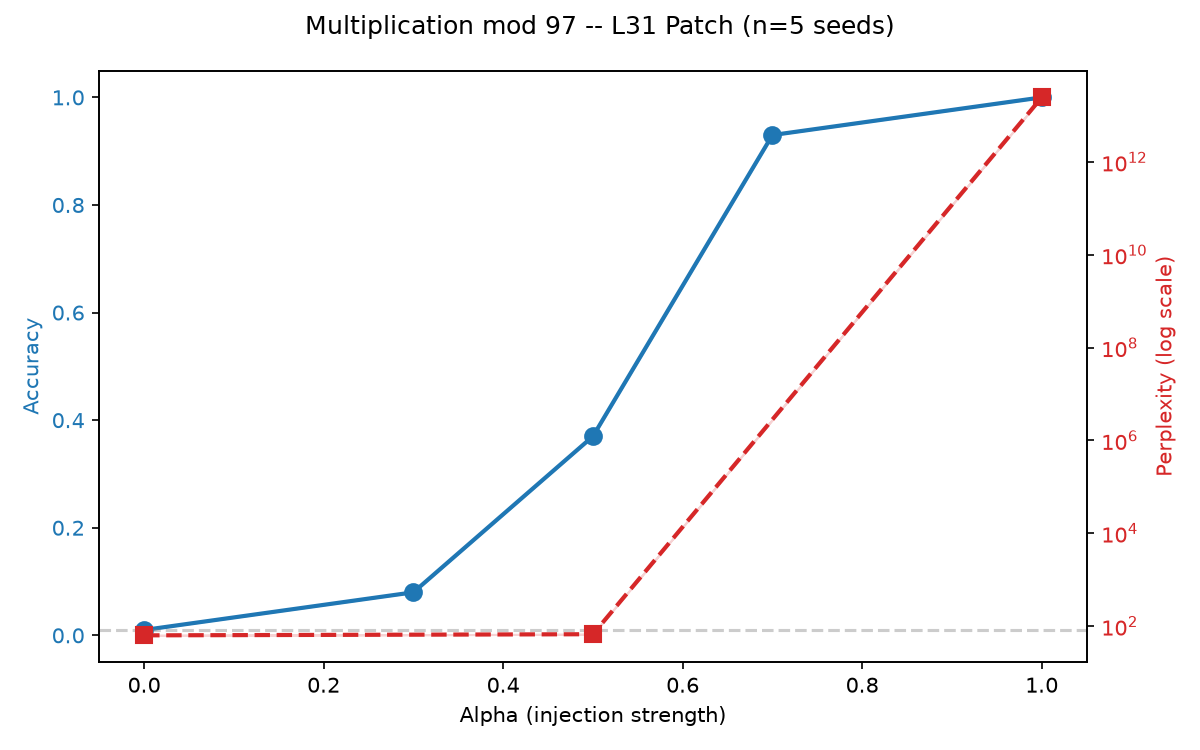
\includegraphics[width=0.75\textwidth]{../artifacts/paper_figures/alpha_sweep_multiply.png}
  \caption{\textbf{L31 $\alpha$-sweep for multiplication mod~97.}
  Same format as Figure~\ref{fig:alpha_add}.  Accuracy reaches $1.0$ at
  $\alpha=1.0$ with a steeper climb after $\alpha=0.5$ compared to addition.}
  \label{fig:alpha_mult}
\end{figure}

\section{Cross-task Comparison}
\label{app:cross_task}

Figure~\ref{fig:cross_task} compares addition and multiplication accuracy
side-by-side, highlighting the consistent pattern.

\begin{figure}[ht]
  \centering
  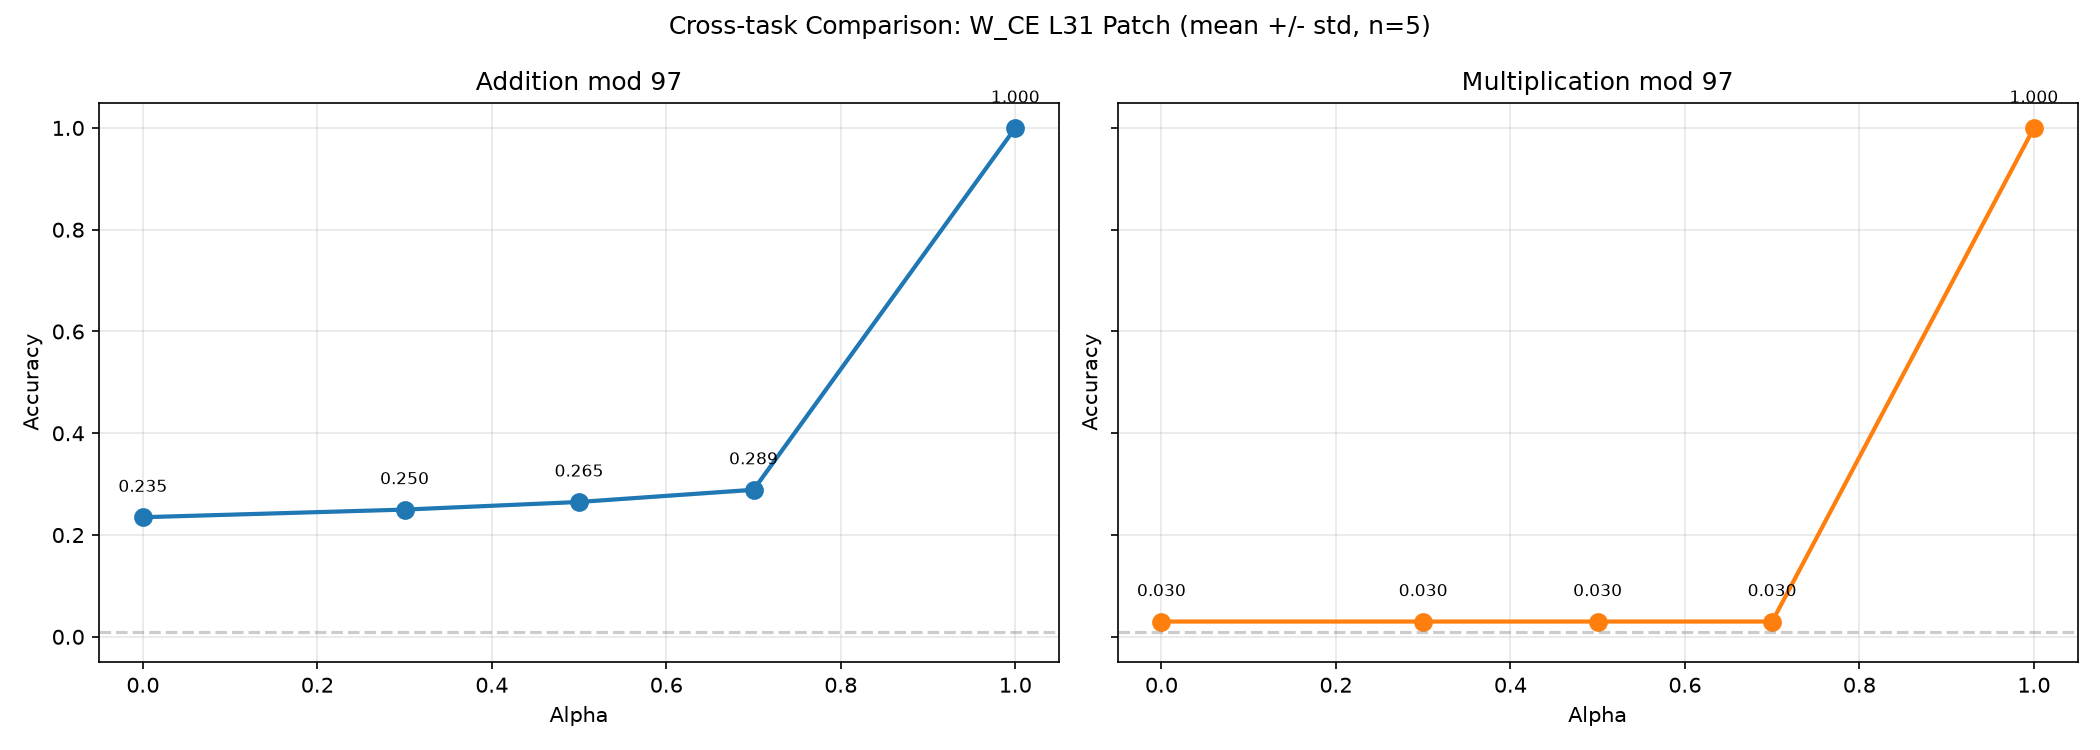
\includegraphics[width=0.85\textwidth]{../artifacts/paper_figures/cross_task_comparison.png}
  \caption{\textbf{Cross-task comparison.}
  Addition (blue) and multiplication (orange) accuracy across $\alpha$ values.
  Both tasks reach $1.0$ at $\alpha=1.0$; multiplication lags at intermediate
  $\alpha$ values.}
  \label{fig:cross_task}
\end{figure}

\section{Failure-mode Details}
\label{app:failure}

\paragraph{SVCCA + Noise Injection.}
Prior work used SVCCA with $k=20$ to compare residual-stream representations.
Raw CCA on 128-dimensional (Small) vs.\ 512-dimensional (Big) activations
over $N=2823$ test points overfits to $\sim 1.0$; dimensionality reduction
to $k=20$ gives meaningful alignment scores.  Layer-by-layer SVCCA reveals
that layers align by position, not cross-functionally
(e.g., Small[1] $\leftrightarrow$ Big[5] $= 0.835$).

Noise injection experiments calibrated to the embedding norm ($\sim 22.65$)
used $\sigma \in \{0.05, 0.10, 0.20, 0.50\}$---higher $\sigma$ values
($0.5, 1.0, 2.0$) completely destroy signal.  Steering vectors become
indistinguishable from random directional vectors when cosine similarity
drops below $\sim 0.7$.

\paragraph{Clean Experiment (Small $\rightarrow$ Big).}
A linear projection was trained from Small ($d=128$) to Big ($d=512$) using
MSE with the same tokenizer (direct token IDs 0--96).  Despite matching
tokenizers, testing on natural-language prompts failed, establishing that
tokenizer mismatch is not the primary barrier to transfer.

\paragraph{Embed Patch.}
Bypassing Phi-2's BPE tokenizer by inserting $W_{\text{emb}}(h_{\text{grokked}})$
directly as inputs\_embeds achieves cosine similarity $0.82$ with the
natural embeddings but near-zero task accuracy ($0.01$).  This confirms
that representational similarity does not imply functional transfer.

\paragraph{Multi-layer injection.}
Injecting the projected state at 5 layers simultaneously (L2, L8, L14, L20,
L26) with per-layer projection matrices $W_{\text{layer}}$ degrades accuracy
below the single-layer L10 baseline ($0.105$ at $\alpha=0.3$).  Per-layer
$W$ matrices are approximately equal to a single shared $W$, confirming
that layer-specific alignment does not matter.

\paragraph{Nonlinear adapter.}
A two-layer MLP ($2560 \rightarrow 2560 \rightarrow 2560$) between $W(h)$
and the frozen lm\_head achieves the same accuracy as a linear adapter
($1.0$).  Since two linear layers compose into one linear transformation,
this confirms the bottleneck is not in the projection's expressivity.

\section{Single-template Probe on L31}
\label{app:probe_final}

A logistic regression probe (Linear $2560 \rightarrow 97$) trained on
Phi-2's L31 activations from a single prompt template
(\texttt{"\# ({a} + {b}) \% 97 ="}) achieves $0.71$ accuracy---the same
value as the Phi-2-to-Phi-2 probe in Figure~\ref{fig:cos_probe}---well above
random ($0.01$) but below the grokked model's $1.0$.
This confirms that L31 activations are partially linearly separable under the
standard template, though template sensitivity remains critical:
generalization to diverse natural language templates is substantially weaker
(Appendix~\ref{app:failure}).

\section{Cross-model Probe (Bypassing Tokenizer)}
\label{app:crossmodel}

For models with number-splitting BPE (e.g., Qwen2-Math-1.5B, which splits
87/97 numbers), lm-head-based evaluation is impossible because only 10
unique token outputs exist for 97 classes.  We bypass this by training a
logistic regression probe on $W_{\text{CE}}$-injected last-layer hidden
states.  At $\alpha=1.0$, both Phi-2 L31 and Qwen2-Math-1.5B L27 achieve
probe accuracy $\geq 0.999$, confirming that the injected Fourier features
dominate the residual regardless of target model architecture.

\section{Per-seed Data}
\label{app:seeds}

All five seeds (42--46) produce indistinguishable accuracy values (zero
variance at reported precision) for both addition and multiplication.
Perplexity variance across seeds is negligible ($\sigma < 0.01$ PPL at
$\alpha=0.5$).  Raw weight matrices differ numerically (max element-wise
difference $\sim 0.7$ for addition, $\sim 1.3$ for multiplication),
confirming that the zero accuracy variance is a property of the 97-class
decision boundary, not a seed propagation error.

\begin{table}[ht]
  \centering
  \caption{Per-seed perplexity at $\alpha=0.5$.}
  \label{tab:seed_ppl}
  \begin{tabular}{lcc}
    \toprule
    Seed & Addition PPL & Multiplication PPL \\
    \midrule
    42 & 65.88 & 66.88 \\
    43 & 65.89 & 66.88 \\
    44 & 65.88 & 66.88 \\
    45 & 65.87 & 66.88 \\
    46 & 65.91 & 66.88 \\
    \midrule
    Mean~$\pm$~Std & $65.89 \pm 0.01$ & $66.88 \pm 0.00$ \\
    \bottomrule
  \end{tabular}
\end{table}

\end{document}
